\documentclass[fleqn,10pt]{article}
\usepackage[T1]{fontenc}
\usepackage[utf8]{inputenc}
\usepackage[spanish,es-tabla]{babel}
\usepackage{helvet}
\renewcommand{\familydefault}{\sfdefault}
\linespread{1.2}

\usepackage{fullpage}
\usepackage{graphicx}
\usepackage{subcaption}
\usepackage{caption}
\usepackage[table]{xcolor}
\usepackage{amsmath}
\usepackage{amssymb}
\usepackage{amsthm}
\usepackage{fancyvrb}
\usepackage{listings}
\usepackage{lipsum,multicol}
\usepackage{framed}
\usepackage{enumerate}
\usepackage[shortlabels]{enumitem}

\usepackage{tabularx}
\usepackage{ltablex}


\parindent0in
\pagestyle{plain}
\thispagestyle{plain}

\newcommand{\nombre}{Navarro Serrano, Jairo Alejandro}
\newcommand{\codigo}{217294601}
\newcommand{\institucion}{CU de CS Exactas e Ingenierías, Universidad de Guadalajara}
\newcommand{\carrera}{Ingeniería en Informática}
\newcommand{\materia}{I5891: Seminario de Solución de Bases de Datos}
%\newcommand{\trabajo}{trabajo}
\newcommand{\fecha}{\today}
\newcommand{\titulo}{Scripts en Python}

\definecolor{light-gray}{gray}{0.95}

\renewcommand{\lstlistingname}{Código fuente}
\lstset{
	basicstyle=\ttfamily,
    frame=tb, % draw a frame at the top and bottom of the code block
    tabsize=4, % tab space width
    showstringspaces=false, % don't mark spaces in strings
    numbers=left, % display line numbers on the left
    commentstyle=\color{green}, % comment color
    keywordstyle=\color{blue}, % keyword color
    stringstyle=\color{red} % string color
}

\begin{document}
\textbf{\nombre}; \textbf{\codigo} \hfill \textbf{\fecha} \\
\textbf{\institucion} \\
\textbf{\carrera} \\ 
\textbf{\materia, sección D12} \\
\smallskip\hrule\bigskip
\begin{center}
\Large{\textbf{\titulo}}
\end{center}

En esta practica se desarrolló un programa escrito en Python 3 para la gestión de la base de datos Invernadero. En este se añade y busca información conectado a través de una conexión y un cursor usando la librería mysql.connector. Para este documento se ejemplificará el uso del script \texttt{registro.py}, \texttt{menuregistro.py} y la aplicación principal \texttt{app.py}.\par
A continuación se presenta el código de \texttt{app-.py}, el cuerpo principal del programa. En este se puede ver el menú principal de opciones, las declaraciones de cursor y conexión a la base de datos deseada y además las librerías (existentes y creadas) que son usadas en el programa.
\begin{lstlisting}[language=python,caption={\texttt{app.py}.}]
import mysql.connector
from dueno import Dueno
from menudueno import MenuDueno
from menuinvernadero import MenuInvernadero
from menuusuario import MenuUsuario
from menuplanta import MenuPlanta
from menuregistro import MenuRegistro

conexion=mysql.connector.connect(user='alejandro',password='12345',
database='invernadero')
cursor=conexion.cursor()

while True:
    print("1) Menu dueno")
    print("2) Menu invernadero")
    print("3) Menu usuario")
    print("4) Menu planta")
    print("5) Menu registro")
    print("0) Salir")
    op=input("Seleccion: ")

    if   op=="1":
        menuD=MenuDueno(conexion,cursor)
    elif op=="2":
        menuI=MenuInvernadero(conexion,cursor)
    elif op=="3":
        menuU=MenuUsuario(conexion,cursor)
    elif op=='4':
        menuP=MenuPlanta(conexion,cursor)
    elif op=='5':
        menuR=MenuRegistro(conexion,cursor)
    elif op=="0":
        break
    else:
        print("No Valido")
\end{lstlisting}

A este código se le está vinculado la clase \texttt{menuregistro.py}, cuyo código a continuación:
\begin{lstlisting}[language=python,caption={\texttt{menuregistro.py}.}]
from registro import Registro
from datetime import datetime,date

class MenuRegistro:
    def __init__(self,conexion,cursor):
        self.registro=Registro(conexion,cursor)

        while True:
            print("1) Agregar registro")
            print("2) Buscar por planta")
            print("0) Regresar")
            op=input("Seleccion: ")

            if   op=='1':
                self.agregar()
            elif op=='2':
                self.buscar()
            elif op=='0':
                break
            else:
                print("No valido")

    def agregar(self):
        dia=input("Dia: ")
        mes=input("Mes: ")
        year=input("Anho: ")
        fecha=date(int(year),int(mes),int(dia))
        luz=input("Luz (lm): ")
        ph=input("pH: ")
        humedad=input("Humedad %: ")
        co2=input("CO2 %: ")
        id_planta=input("Id planta: ")
        self.registro.agregar(fecha,luz,ph,humedad,co2,id_planta)

    def buscar(self):
        id_planta=input("Id planta: ")
        resultados=self.registro.buscar(id_planta)
        for p in resultados:
            print(p)
            #print("{0:2} {1:10} {2:10}".format(p[0],p[1],str(p[2])))
            print("{0:2} {1:10} {2:3} {3:3} {4:3} {5:3} {5:3}".
            format(p[0],str(p[1]),p[2],p[3],p[4],p[5],p[6]))
\end{lstlisting}
En esta clase se capturan y guardan los datos del registro a la respectiva tabla \texttt{registro} en la base de datos invernadero. En la clase registro se encuentran los movimientos necesarios del cursor para la escritura, con la posibilidad de ignorar la entrada sí la id\_planta no existe.
\begin{lstlisting}[language=python,caption={\texttt{registro.py}.}]
class Registro:
    def __init__(self,conexion,cursor):
        self.conexion=conexion
        self.cursor=cursor

    def agregar(self,fecha,luz,ph,humedad,co2,id_planta):
        insertar=("INSERT INTO registro(fecha,luz,ph,humedad,co2,id_planta) 
        VALUES(%s,%s,%s,%s,%s,%s)")
        self.cursor.execute(insertar,(fecha,luz,ph,humedad,co2,id_planta))
        self.conexion.commit()

    def buscar(self,id_planta):
        select=("SELECT * FROM registro WHERE id_planta = %s")
        self.cursor.execute(select,(id_planta,))
        return self.cursor.fetchall()
\end{lstlisting}

\begin{figure}[h]
  \begin{center}
    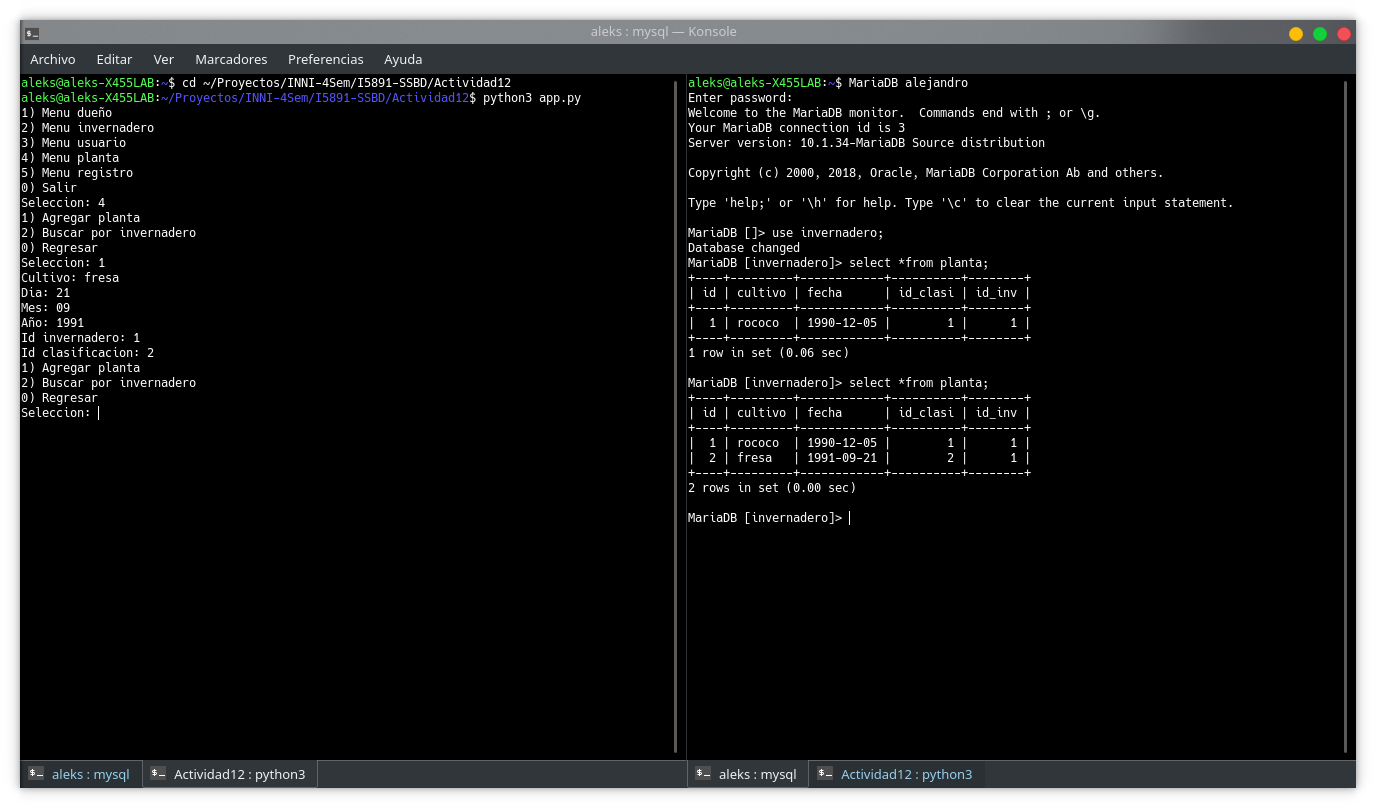
\includegraphics[scale=0.4]{./pics/01.png}
  \end{center}
  \vspace{-20pt}
  \caption{Agregando una planta a la tabla planta.}
  \vspace{-10pt}
\end{figure}

\begin{figure}[h]
  \begin{center}
    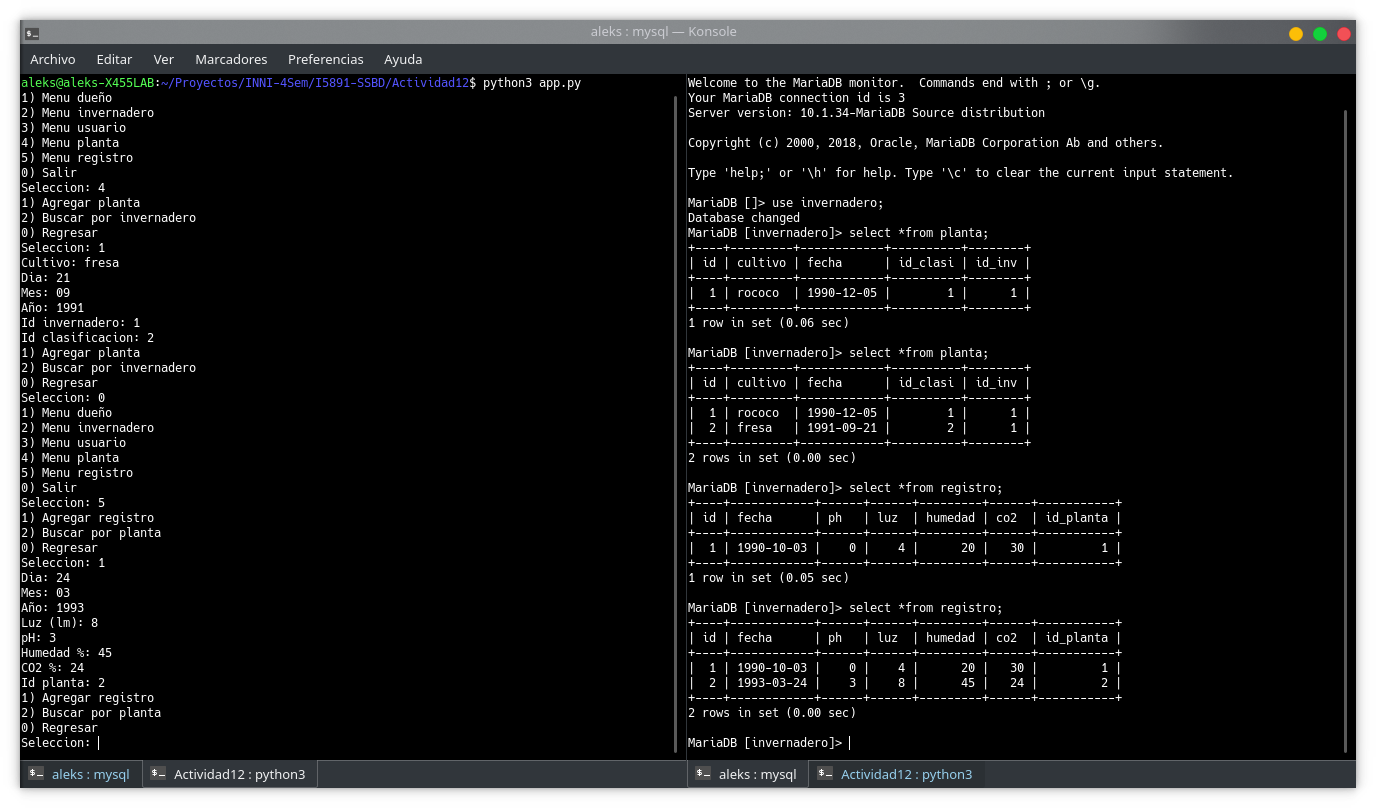
\includegraphics[scale=0.4]{./pics/02.png}
  \end{center}
  \vspace{-20pt}
  \caption{Agregando un registro a la planta con id 2 a la tabla registro.}
  \vspace{-10pt}
\end{figure}

\end{document}
